\documentclass{ustlfile}
\pagenumbering{Roman}
\title{本科生毕业论文LaTeX模板}
\date{}
\author{}
\begin{document}
\maketitle % 生成标题
\begin{abstract}% 中文摘要部分
    模板说明请自行删除\par
    LaTeX发行版:TeXLive 2020\par
    本模板以《辽宁科技大学本科生毕业设计(论文)撰写规范(修订)》为参考编写,撰写规范为2020年版本,以后若有更新,请搜索我的GitHub(BasinChen),也欢迎各位同行
    对我的模板批评指正,若有改动,可以发邮件到421958880@qq.com或发Pull Requests。模板中使用了一些来自于LaTeX论坛的开源代码及图片,在此对原作者表示感谢!\par
    模板中的标题可以按意愿自行更改,但在非必须的情况下请不要更改导言区以及其他命令的配置。\par
    本模板参考文献的引用使用了bib文件的方法,配合EndNote较为简便快捷。\par
    由于学校规定,封面页统一打印,故此模板不提供封面页。若有需要,可以与我讨论,也欢迎直接在GitHub发布Pull Requests。\par
    由于本人能力有限,模板有瑕疵之处在所难免,本模板会不断更新,感谢各位提供支持!\par
    \keywords{关键词1,关键词2}% 填写中文关键词
\end{abstract}
\newpage
\begin{center}
  \erhao {English Title}%英文标题  
\end{center}
\renewcommand{\abstractname}{\sanhao{Abstract}}
\begin{abstract}% 英文摘要部分
    Please delete the template description by yourself.
    LaTeX distribution: TeXLive 2020 \par
    This template is compiled for the reference of the specification (Revision) of Graduation Design (Thesis) for Undergraduates of Liaoning University of Science and Technology, 
    and the specification is written for 2020 version.
     If there is any update, please search my GitHub (BasinChen), and you are also welcome to criticize and criticize my template.
      If there is any change, you can send email to 421958880@qq.com or Pull Requests.Some open source code and pictures from LaTeX forum are used in the template. 
     Thanks to the original author!\par
    The headers in the template can be changed as desired, but do not change the configuration of the introduction area and other commands unless it is necessary.\par
    The reference of this template USES the method of BIB file, which is simple and fast with EndNote.\par
    Due to the school regulation, the cover page is printed uniformly, so the template does not provide the cover page.
    Please feel free to discuss Pull Requests with me and post them directly on GitHub.\par
    Due to my limited ability, it is hard to avoid defects in the template. This template will be updated constantly. Thank you for your support!\par
  \ekeywords{KeyWords1, KeyWords2}% 填写英文关键词
\end{abstract}
\newpage
\tableofcontents% 生成目录
\newpage
\pagenumbering{arabic}
\setcounter{page}{1}% 重置计数器
%% 正文开始
\section{一级标题}
(这是一级标题示例正文内容,以下随机文本请自行删除)

\zhlipsum[1]
\subsection{二级标题}
(这是二级标题示例正文内容,以下随机文本请自行删除)

\zhlipsum[2]
\subsubsection{三级标题}
(这是三级标题示例正文内容,以下随机文本请自行删除)

\zhlipsum[2]
\paragraph{四级标题}

(这是四级标题示例正文内容)

\newpage

\section{公式的编写}
\subsection{带序号的公式}
\begin{equation}
    u(t)=k_p\left[ e(t)+\frac{1}{T_1}\int e(t)\mathrm{d}t +T_D\frac{\mathrm{d}e(t)}{\mathrm{d}t} \right]
\end{equation}
\subsection{不带序号的公式}
$E=mc^2$
\[ F=ma \]

\section{表格(三线表)}
\begin{table}[htbp] 
\setlength{\abovecaptionskip}{0.cm}
\setlength{\belowcaptionskip}{-0.9cm}
    \caption{示例表格} 
    \begin{center}
        \begin{tabular}{lcl} 
     \toprule 
     这是第一行第一列 & 这是第一行第二列 & 这是第一行第三列 \\ 
     \midrule 
    。。 & 。。 & 。。 \\ 
    。。 & 。。 & 。。 \\ 
    。。 & 。。 & 。。 \\ 
     \bottomrule 
    \end{tabular} 
    \end{center}
   \end{table}
   \section{图片插入}
   \subsection{单个图片}
   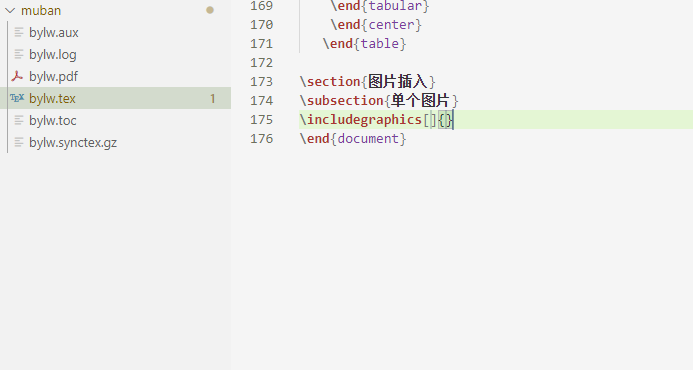
\includegraphics[scale=0.8]{f1.PNG}
   \newpage
   \subsection{有标题的图片}
   
   \begin{figure}[h]
       \centering %居中显示
       \caption{图片的标题}
       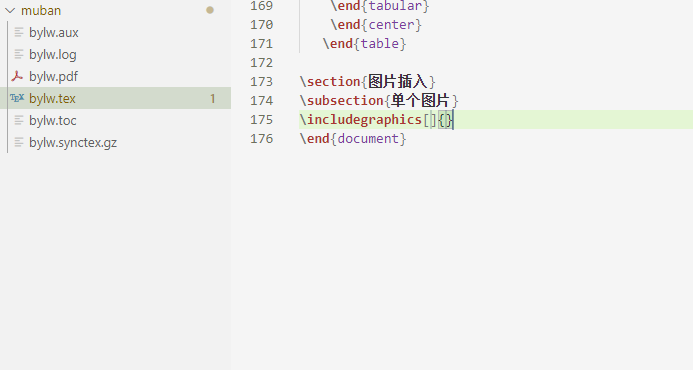
\includegraphics[scale=0.8]{f1.PNG}
       \end{figure}
   
   \subsection{多个图片表格}
   
   \begin{figure}[!htp]
       \begin{floatrow}
         \ffigbox[\FBwidth]{
           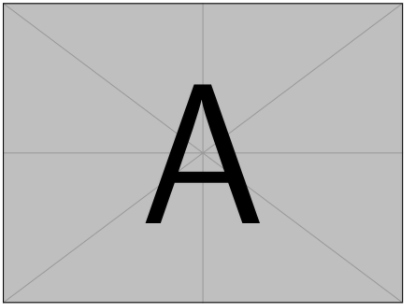
\includegraphics[scale=0.8]{A.PNG}
           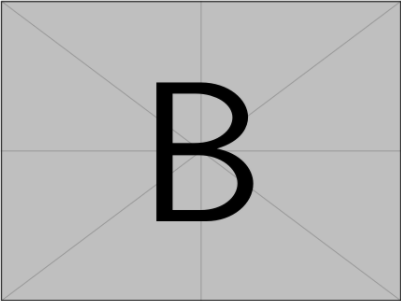
\includegraphics[scale=0.8]{B.PNG}
         }{\caption{共享题注}\label{sharefig:a}}
       \end{floatrow}
     \end{figure}
   
   \begin{figure}[!htp]
       \begin{floatrow}
         \ffigbox[\FBwidth]{
           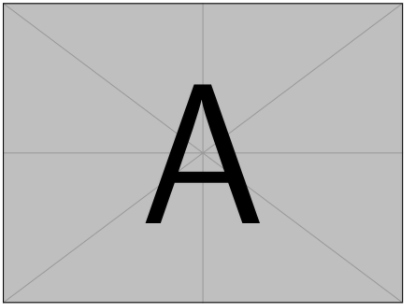
\includegraphics[scale=0.8]{A.PNG}
         }{\caption{独立题注}\label{sepfig:a}}
         \ffigbox[\FBwidth]{
           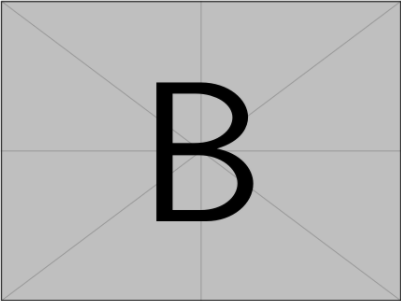
\includegraphics[scale=0.8]{B.PNG}
         }{\caption{独立题注}\label{sepfig:b}}
       \end{floatrow}
     \end{figure}
   
     \begin{figure}[!htp]
       \begin{floatrow}
         \ffigbox[\textwidth]{
           \begin{subfloatrow}[2]
             \ffigbox[\FBwidth]{
               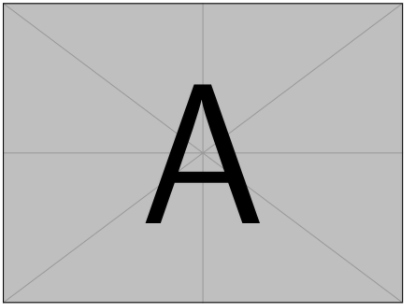
\includegraphics[scale=0.8]{A.PNG}
             }{\caption{子题注}\label{subfig:a}}
             \ffigbox[\FBwidth]{
               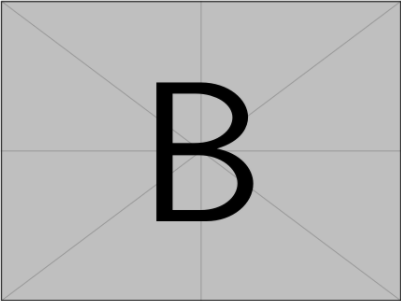
\includegraphics[scale=0.8]{B.PNG}
             }{\caption{子题注}\label{subfig:b}}
           \end{subfloatrow}
         }{\caption{共享题注带子题注}\label{fig:sub}}
       \end{floatrow}
   \end{figure}
   
   \begin{figure}[!htp]
       \ffigbox[\textwidth]%
       {%
           \begin{subfloatrow}[2]%useFCwidth
           \ffigbox[\FBwidth]{
               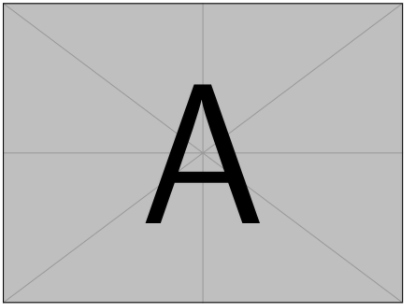
\includegraphics[scale=0.8]{A.PNG}
           }{\caption{子题注1}\label{trifig:a}}
           \ffigbox[\FBwidth]{
               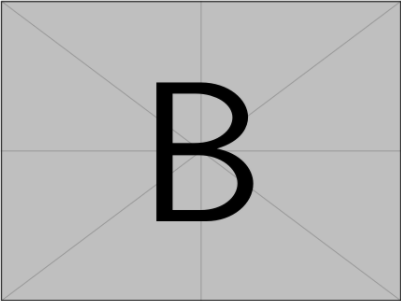
\includegraphics[scale=0.8]{B.PNG}
           }{\caption{子题注2}\label{trifig:b}}
           \end{subfloatrow}    
           \begin{subfloatrow}[2]%useFCwidth      
           \ffigbox[\FBwidth]{
               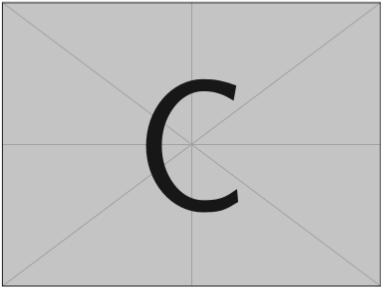
\includegraphics[scale=0.8]{C.PNG}
           }{\caption{子题注3}\label{trifig:c}}
           \ffigbox[\FBwidth]{
               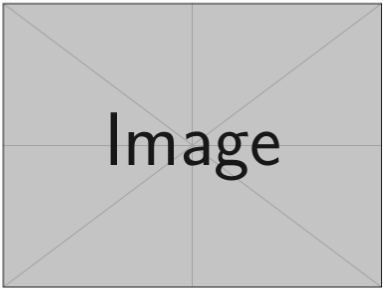
\includegraphics[scale=0.8]{D.PNG}
           }{\caption{子题注4}\label{trifig:d}}
           \end{subfloatrow}
       }{\caption{四个子图}\label{trifig}}
   \end{figure}
   \newpage
   \ctexset{
section = {
format = \sanhao\center\bfseries,
}
}
   \addcontentsline{toc}{section}{\hspace{-0.65cm}总结与展望}
   \clearpage
 \section*{总结与展望}
 \newpage
   用下面那样的命令引用引用参考文献
   \upcite{RN1}
   
   
   引用参考文献
   \upcite{RN2}
   
   
   引用参考文献
   \upcite{RN3}
   
   引用参考文献
   \upcite{RN4}
   
   引用参考文献
   \upcite{RN5}
   
   引用参考文献
   \upcite{RN6}
   
   不能这样引用参考文献
   \cite{RN7}
   \newpage  
    \addcontentsline{toc}{section}{\hspace{-0.65cm}致谢}
\clearpage
   \section*{致谢}

   这是致谢的内容
   \newpage  
    \addcontentsline{toc}{section}{\hspace{-0.65cm}参考文献}
\clearpage
   \bibliography{Library}
      \newpage
      \addcontentsline{toc}{section}{\hspace{-0.65cm}附录}
\clearpage
   \section*{附录}
   这是附录的内容


\end{document}
